\documentclass{scrartcl}
\usepackage[utf8]{inputenc}
\usepackage[english]{babel}
\usepackage{caption}
\usepackage{listings}
\usepackage{pdfpages}
\usepackage{amsmath,amssymb}
\usepackage{bm}

\newcommand{\qed}{\hfill $\blacksquare$}

\lstset{frame=single,keepspaces=true,captionpos=b}

\title{Homework 10 - Dimensionality Reduction}
\author{Arne Sachtler - \textit{Registration Number: 03692662}}
\date{\today}
\subtitle{IN2064 Machine Learning}

\begin{document}
\maketitle

\section{Problem 1} % (fold)
\label{sec:problem_1}
First we use the Langrangian formalism in order to compute our new vector $u_{M+1}$
\begin{equation}
	u_{M+1} = \underset{u}{\arg \max}\left(L(u, \lambda_0, \ldots, \lambda_M)\right)=  \underset{u}{\arg \max}\left(  u^\top Su + \lambda_0 (1-u^\top u) +\sum_{i=1}^{M} \lambda_i u_i^\top u \right) \, .
\end{equation}
Computing the derivative we obtain
\begin{equation}
	\left(\frac{\partial L}{\partial u}\right)^\top = 2u^\top S - 2 \lambda_0u^\top + \sum_{i=1}^{M}\lambda_i u_i^\top \overset{!}{=} 0
\end{equation}
Let's consider left multiply the equation with the last eigenvector $u_M$ and $u$ will be called $u_{M+1}$ for consistency reasons.
This multiplication is allowed as $u_M$ is always non-zero.
\begin{eqnarray}
	0 &=& u_M^\top \left(2S u_{M+1} - 2 \lambda_0u_{M+1} + \sum_{i=1}^{M}\lambda_i u_i\right)\\
	&=& 2u_M^\top S u_{M+1} - 2 \lambda_0u_M^\top u_{M+1} + \sum_{i=1}^{M}\lambda_i u_M^\top u_i\\
	&=& u_M^\top S u_{M+1} - \lambda_0 u_M^\top u_{M+1}\\
	&=& S u_{M+1} - \lambda_0u_{M+1}
\end{eqnarray}
Here the orthogonality property
\begin{equation}
	\forall i,j\in\left\{1 \ldots M\right\}: i \neq j \implies u_i^\top u_j = 0
\end{equation}
was used.
Finally we get the eigenvalue problem 
\begin{equation}
	S u_{M+1} = \lambda_0 u_{M+1} \, .
\end{equation}
\qed



% section problem_1 (end)

\section{Problem 2} % (fold)
\label{sec:problem_2}
First let us recap a fundamental rule for linear transformation of Gaussian random variables. Given a normal-distributed random variable $X$ with mean $\bm{\mu}_X$ and variance $\bm{\Sigma}_X$, more formally
\begin{equation}
	X \sim \mathcal{N}(\bm{\mu}_X, \bm{\Sigma}_X) \, ,
\end{equation}
we can construct a new normal-distributed random variable $Y$ using the linear transformation $\mathbf{y} = \mathbf{A} \mathbf{x}$.
Then, the constructed random variable $Y$ is distributed as 
\begin{equation}
	Y \sim \mathcal{N}(\bm{\mu}_Y, \bm{\Sigma}_Y) = \mathcal{N}(\mathbf{A}\bm{\mu}_X, \mathbf{A}^\top \bm{\Sigma}_X \mathbf{A})\, .
\end{equation}
It follows that
\begin{equation}
	E\left[Y\right] = \bm{\mu}_Y = \mathbf{A}\bm{\mu}_X
\end{equation}
and
\begin{equation}
	Var\left[Y\right] = \bm{\Sigma}_Y = \mathbf{A} \bm{\Sigma}_X \mathbf{A}^\top \, .
\end{equation}


Given the maximum likelihood estimates $\bm{\mu}_{ML}$, $\bm{W}_{ML}$ and $\bm{\Phi}_{ML}$ we know the data $X$ is distributed as
\begin{equation}
	X \sim \mathcal{N}(\bm{\mu}_{ML}, \mathbf{M}_{ML}\mathbf{M}_{ML}^\top + \bm{\Phi}_{ML}) \, .
\end{equation}
Now let $Y$ be the random variable of the linearly transformed data with the transformation rule $\mathbf{y} = \mathbf{A}\mathbf{x}$.
Using the rules for linear transformation of Gaussian random variables we get for the expected value
\begin{equation}
	E\left[Y\right] = \mathbf{A}\bm{\mu}_{ML}
\end{equation}
and for the variance
\begin{eqnarray}
	Var\left[Y\right] &=& \mathbf{A} \left(\mathbf{M}_{ML}\mathbf{M}_{ML}^\top + \bm{\Phi}_{ML}\right)\mathbf{A}^\top\\
	&=& \mathbf{A} \mathbf{W}_{ML} \mathbf{W}_{ML}^\top \mathbf{A}^\top + \mathbf{A} \bm{\Phi}_{ML} \mathbf{A}^\top\\
	&=& \mathbf{A}\mathbf{W}_{ML}\left(\mathbf{A}\mathbf{W}_{ML}\right)^\top + \mathbf{A} \bm{\Phi}_{ML} \mathbf{A}^\top \, .
\end{eqnarray}
Comparing this to the PPCA formulation we see that the new maximum likelihood estimates for the transformed data space are
\begin{eqnarray}
	\bm{\mu}_{ML}' &=& \mathbf{A} \bm{\mu}_{ML}\\
	\bm{W}_{ML}' &=& \mathbf{A} \bm{W}_{ML}\\
	\bm{\Phi}_{ML}' &=& \mathbf{A} \bm{\Phi}_{ML} \mathbf{A}^\top \, .
\end{eqnarray}

Finally, given that $\bm{\Phi} = \sigma^2 \mathbf{I}$ we apply the transformation $A$:
\begin{equation}
	\bm{\Phi}' = \mathbf{A}\bm{\Phi} \mathbf{A}^\top = \sigma^2 \mathbf{AIA}^\top = \sigma^2 \mathbf{AA}^\top = \sigma^2 \mathbf{I} \, , 
\end{equation}
as $\mathbf{A}$ is orthogonal.\qed

% section problem_2 (end)

\section{Problem 3} % (fold)
\label{sec:problem_3}
Leslie in concept space is
\begin{equation}
	\begin{pmatrix}
		0&3&0&0&4
	\end{pmatrix}\mathbf{V} = \begin{pmatrix}
		1.74 & 2.84
	\end{pmatrix}\, .
\end{equation}
Interpretation: Leslie likes everything, but has a tendency to romantic movies.

% section problem_3 (end)

\section{Problem 4} % (fold)
\label{sec:problem_4}
See the pages attached.
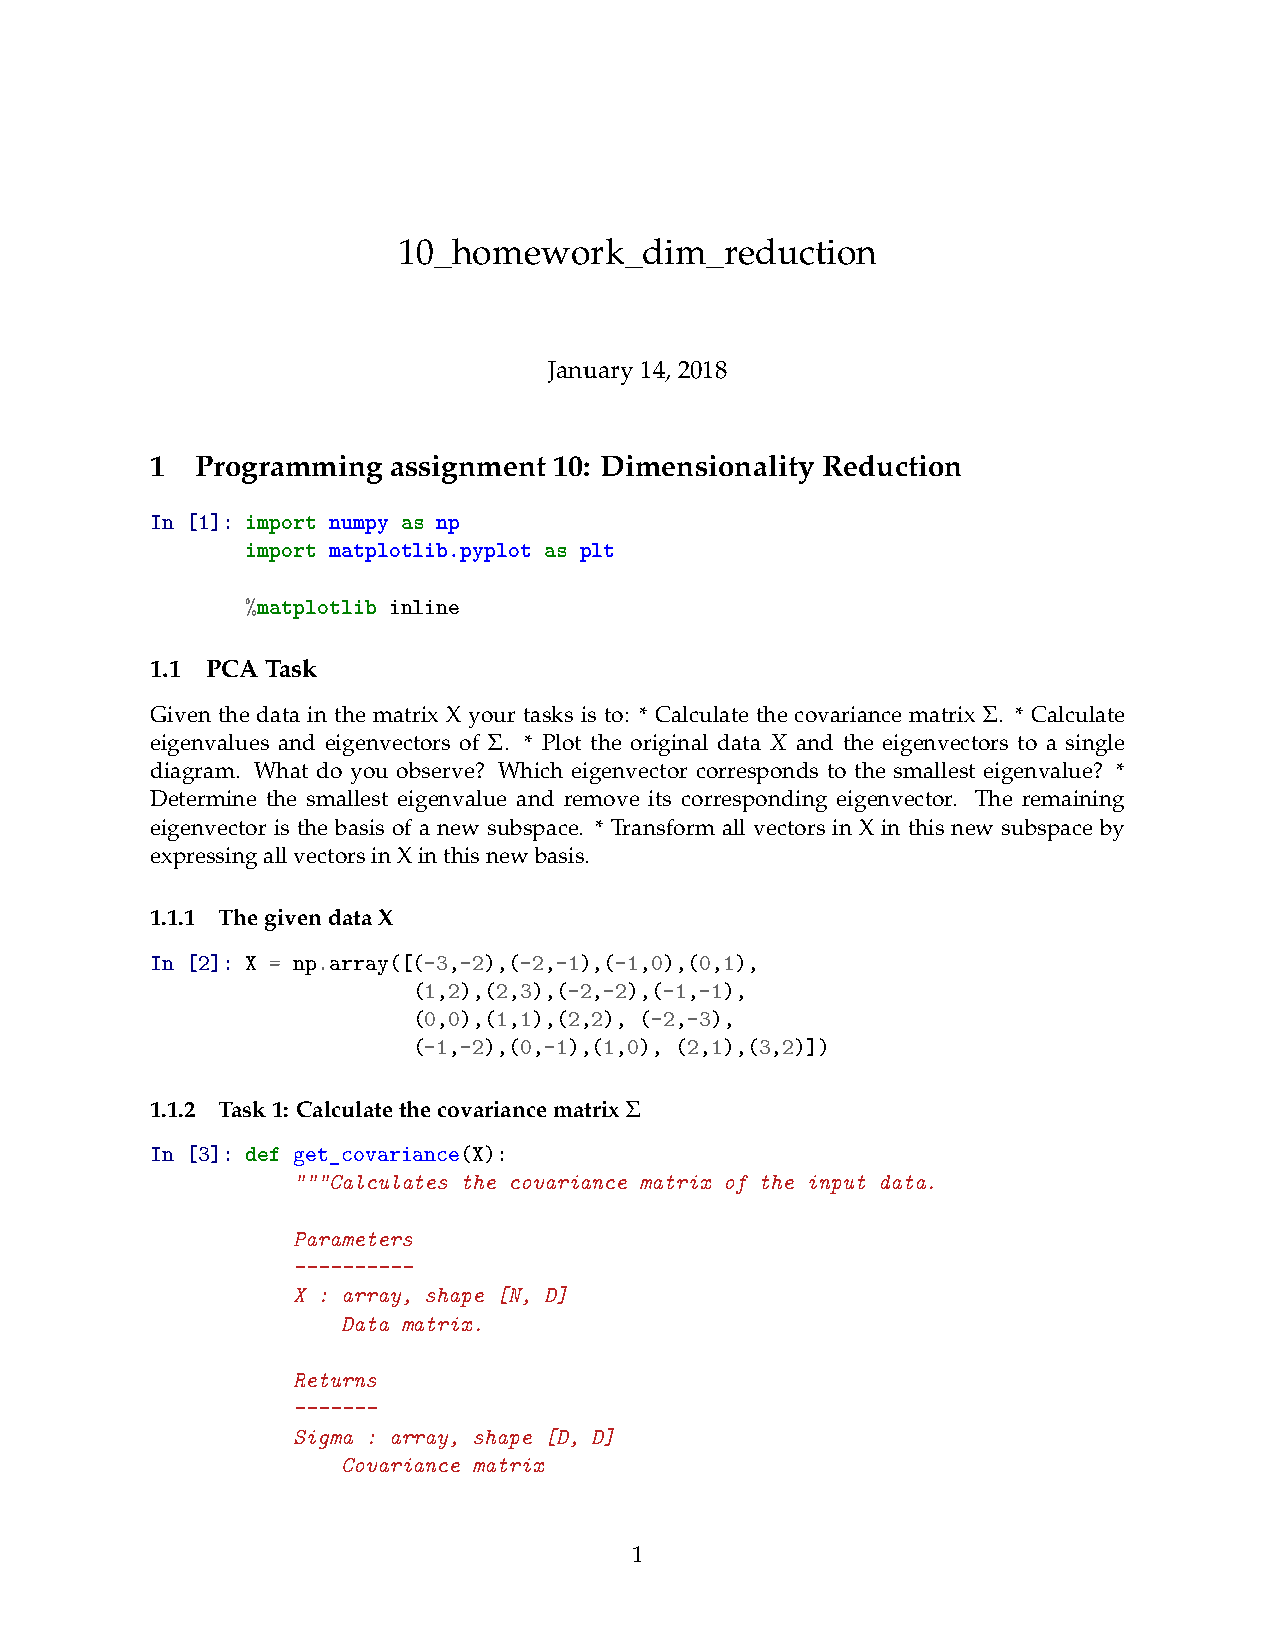
\includepdf[pages=-]{10_homework_dim_reduction.pdf}

% section problem_4 (end)
	
\end{document}
